\chapter{Analysis}
	The most important results of the problem analysis are documented in this chapter.
	
\section{Use Case Model}
	All identified use cases of RaceTrack are described in this section. Each use case is identified by an id in the form of \textbf{UC}n (e.g. UC1, UC2, ...). Use cases are added and removed during development but don't change their ids during the entire development cycle (Reason why some use cases, e.g. UC5, don't exist anymore).

	\subsection{Overview}
		\begin{figure}[H]
			\centering
			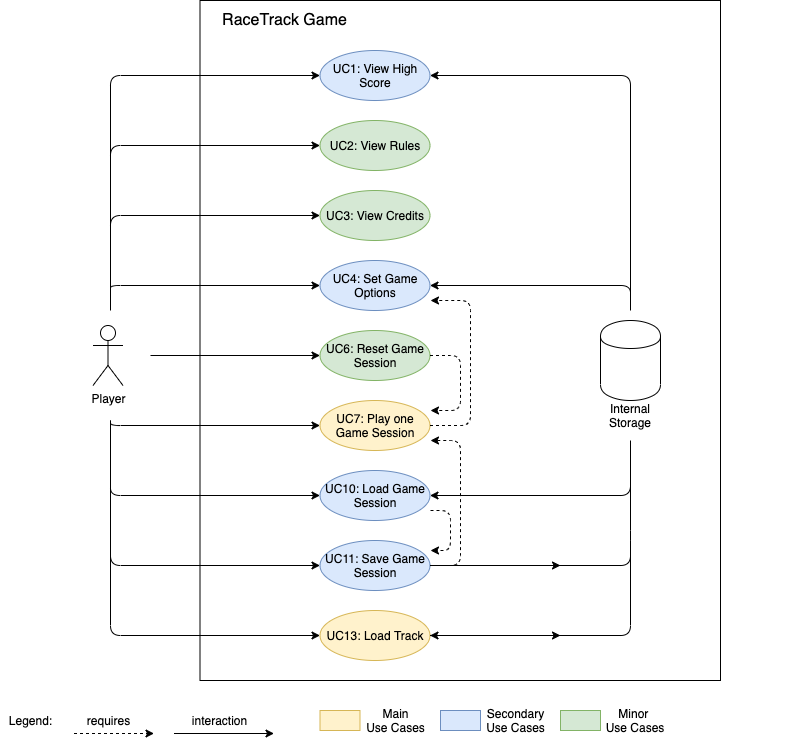
\includegraphics[width=17cm,keepaspectratio,center]{img/Use-Case-Model_Overview.png}
			\caption{Overview of all defined use cases of RaceTrack}
		\end{figure}
		\begin{itemize}
			\item UC6 requires UC7, as there is no session to reset if no session is currently being played.
			\item UC7 requires UC4, as the options for the game session need to be defined by the player before the session can be started.
			\item UC10 requires UC11, as a game session first needs to be saved before it can be loaded again.
			\item UC11 requires UC7, as there is no session to be saved if no session is currently being played.
		\end{itemize}

	\subsection{Main Use Cases}
		
		\subsubsection{Use Case UC7: Play one Game Session}
			\textbf{Scope:} RaceTrack Game \\
			\textbf{Level:} User Goal \\
			\textbf{Primary Actor:} Player \\
			\textbf{Stakeholders and Interests:} \\
			Player: Wants to play one game session of RaceTrack, either alone or with up to three friends. \\
			\textbf{Preconditions:} A track has been loaded (UC10) and the game session has been successfully started with the player's settings (UC4). \\
			\textbf{Success Guarantee:} The game session has been successfully played. Every player has reached the finish line and the high score board is being displayed (UC1). \\
			\textbf{Frequency of Occurrence:} Once for every game session played.
			\newline

			\textbf{Main Success Scenario}
				\begin{enumerate}
					\item The session starts and the system places each player's car on the starting line.
					\item The order of the placement is from the top left to the bottom right.
					\item The first player to start is determined randomly.
					\item The player is given a total of maximum 9 possible moves he can choose for his car during his turn.
					\begin{enumerate}
						\item The possible moves for the player's car are calculated before each turn, based on the player's velocity, previous turns, and potential obstacles on the track (e.g. another player's car).
						\item With each move the player can accelerate, decelerate, or maintain his current velocity.
						\item All available moves the player can take are shown on the track.
					\end{enumerate}
					\item The player chooses his move out of the possible moves.
					\item The player's car drives to the selected position on the track.
					\begin{enumerate}
						\item Once a player reaches the finish line, his placement is saved and can no longer participate in the current race.
					\end{enumerate}
					\textit{Each player repeats steps 4. - 6. for his turn until every player reaches the finish line.}
					\item The session ends and the scores of the just-finished race are displayed.
					\item The players can restart another session with the same settings or return to the main menu.
				\end{enumerate}

			\textbf{Alternative Flows}
				\begin{enumerate}
					\item At any time, a player drives past the track limits:
					\begin{enumerate}
						\item When the \textbf{Go Kart} game mode \textit{(Continue with minimum velocity and no acceleration until the track is reached again)} is selected during game creation:
						\begin{enumerate}
							\item The player's velocity resets.
							\item The player does not accelerate until the track is reached again.
						\end{enumerate}
						\item When the \textbf{Formula One} game mode \textit{Retire from the race} is selected during game creation:
						\begin{enumerate}
							\item The player \textit{crashes} and receives a corresponding notification about it.
							\item The player retires from the race and will not be able to do any more moves during this game session.
						\end{enumerate}
						\item When the \textbf{Bobby Car} game mode \textit{Reset position to last valid point and reset velocity} is selected during game creation:
						\begin{enumerate}
							\item The player \textit{crashes} and receives a corresponding notification about it.
							\item The player's velocity resets.
							\item The player's car resets to his last valid position on the track.
						\end{enumerate}
					\end{enumerate}
					\item At any time, a player can drive to a position already occupied by another player:
					\begin{enumerate}
						\item The game calculates the player's possible moves and realizes that some possible moves are already occupied by another player.
						\item The game will not show the invalid move to the player as one of the next possible moves anymore.
					\end{enumerate}
					\item When \textit{special items} have been selected as an option while starting the game:
					\begin{enumerate}
						\item Special items e.g. boosts or obstacles are being randomly placed across the track.
						\item When driving on to a special item, its special ability will be activated.
					\end{enumerate}
				\end{enumerate}

			\textbf{Special Requirements}
				\begin{itemize}
					\item Recognisable assets. Cars, track limits, special items and the starting/finish line must be easily recognizable.
					\item The car's movement has to be smooth.
					\item It has to be clear which player's move it currently is.
				\end{itemize}

			\textbf{Technology and Data Variations List}
				\begin{itemize}
					\item Player input is entered by a mouse click or keyboard (0-9).
				\end{itemize}

			\textbf{UI Sketch}
				\begin{figure}[H]
					\centering
					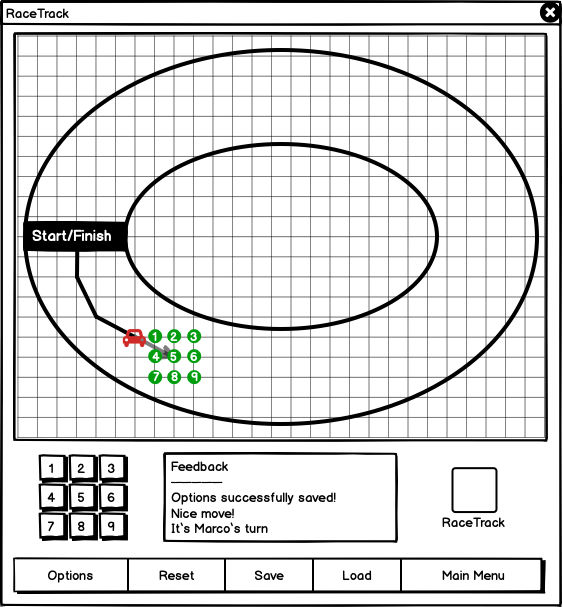
\includegraphics[width=8cm,keepaspectratio,center]{img/Use-Case-Model_UC7_UI-Sketch.png}
					\caption{UI Sketch for Use Case UC7}
				\end{figure}

			\newpage

			\textbf{System Sequence Diagram}
				\begin{figure}[H]
					\centering
					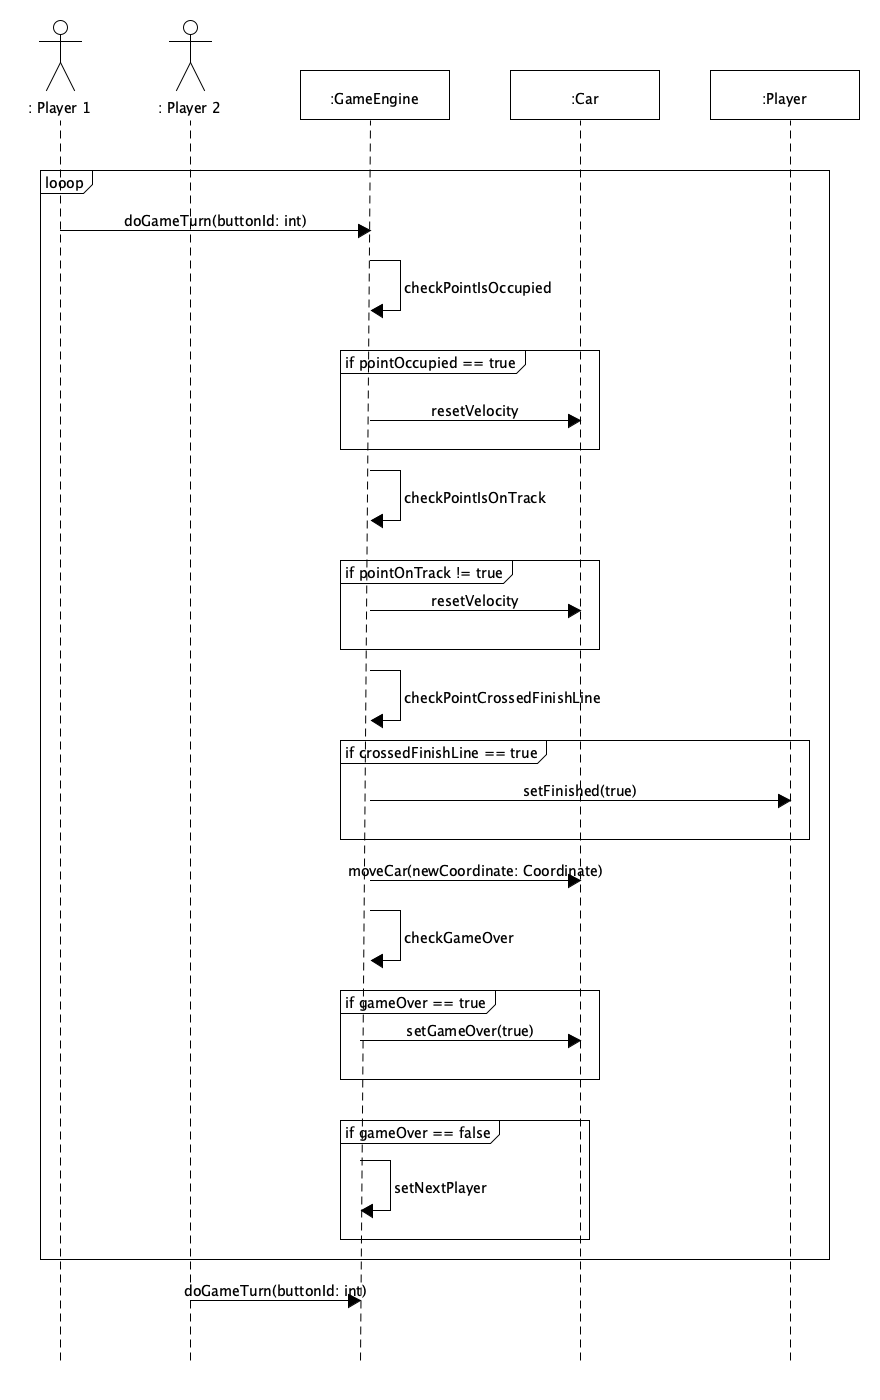
\includegraphics[width=14cm,keepaspectratio,center]{img/Use-Case-Model_UC7_System-Sequence-Diagram.png}
					\caption{System Sequence Diagram of Use Case UC7}
				\end{figure}

			

		\subsubsection{Use Case UC13: Load Track}
			\textbf{Scope:} RaceTrack Game \\
			\textbf{Level:} User Goal \\
			\textbf{Primary Actor:} Player \\
			\textbf{Stakeholders and Interests:} \\
			Player: Wants to load a track from a bitmap image. \\
			\textbf{Preconditions:} A bitmap image that complies with all specifications for a track file (see \textit{Special Requirements}). \\
			\textbf{Success Guarantee:} The track has been successfully loaded into the game and no errors have occurred during the upload process. \\
			\textbf{Frequency of Occurrence:} Once for each new track uploaded.
			\newline

			\textbf{Main Success Scenario}
				\begin{enumerate}
					\item The player selects the \textit{Load Track} entry in the menu.
					\item The player selects a valid bitmap image, which complies with all specifications for a track file (see \textit{Special Requirements}).
					\item The system uploads the selected image into the game and converts it into a track.
					\item The player can upload another track or return to the main menu.
				\end{enumerate}

			\textbf{Alternative Flows}
				\begin{enumerate}
					\item When the player wants to delete an existing track:
					\begin{enumerate}
						\item The player selects an existing track from the list in the tracks menu.
						\item The player confirms the deletion by clicking on the \textit{Delete Track} button.
						\item The system removes the track from the game.
						\begin{itemize}
							\item Default tracks can not be deleted and a comprehensible error message will be displayed when trying so.
						\end{itemize}
					\end{enumerate}
					\item When the verification of the image as a track fails:
					\begin{enumerate}
						\item The game will respond with a comprehensible error message that the image can not be verified as a track.
						\item The player will be allowed to retry the upload process with another image or to return to the main menu.
					\end{enumerate}
				\end{enumerate}

			\textbf{Special Requirements}
				\begin{itemize}
					\item After the file has been uploaded, the track needs to be choosable during the set-up of a new game session (UC4).
					\item The bitmap image needs to comply with these specifications or else the game will not be able to verify it as a track:
					\begin{itemize}
						\item The image must only consist of the following colors \textit{(can still be changed during development)}:
						\begin{itemize}
							\item \textcolor{gray}{\#C5C5C5} : represents the drivable track.
							\item \textcolor{black}{\#000000} / \colorbox{black}{\textcolor{white}{\#FFFFFF}} : represents the starting/finish line.
							\item Every other color will be interpreted as not to be part of the drivable track (out of track boundaries).
						\end{itemize}
						\item The starting/finish line must be placed either vertically or horizontally, it cannot be placed diagonally.
					\end{itemize}

					\newpage

					\item Below is an example of a correct bitmap image:
					\begin{figure}[H]
						\centering
						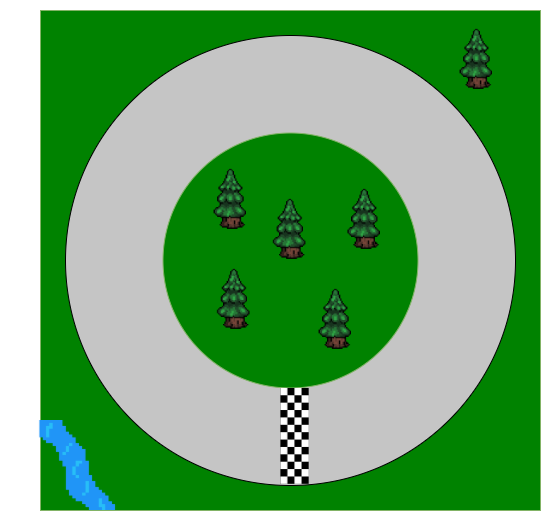
\includegraphics[width=8cm,keepaspectratio,center]{img/Use-Case-Model_UC13_Track-Requirements_Track-Example.png}
						\caption{Example of a valid track to be used in Use Case UC13}
					\end{figure}
				\end{itemize}

			\textbf{Technology and Data Variations List}
				\begin{itemize}
					\item The bitmap file needs to be of the file format \textit{PNG}.
				\end{itemize}

			\textbf{UI Sketch}
				\begin{figure}[H]
					\centering
					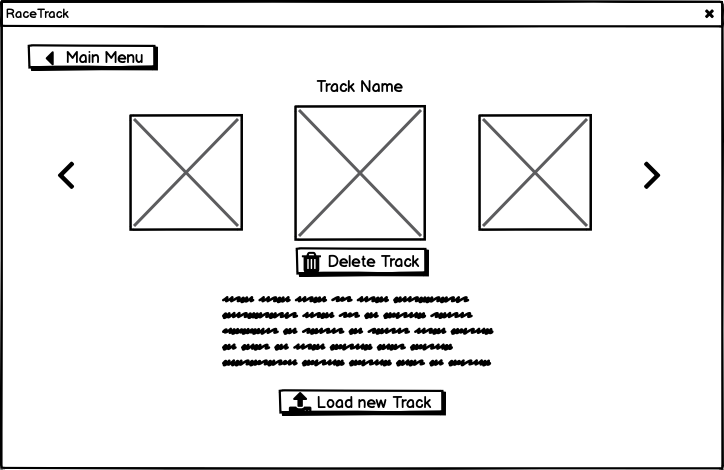
\includegraphics[width=10cm,keepaspectratio,center]{img/Use-Case-Model_UC13_UI-Sketch.png}
					\caption{UI Sketch for Use Case UC13}
				\end{figure}

			\newpage

			\textbf{System Sequence Diagram}
				\begin{figure}[H]
					\centering
					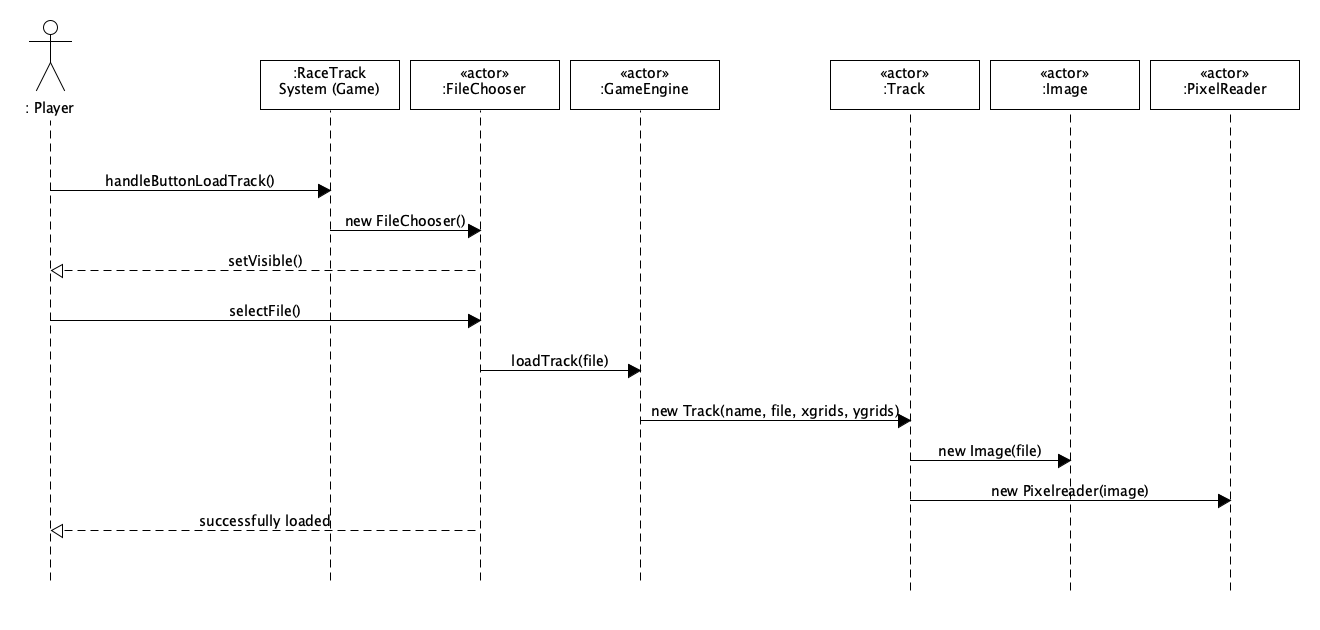
\includegraphics[width=18cm,keepaspectratio,center]{img/Use-Case-Model_UC13_System-Sequence-Diagram.png}
					\caption{System Sequence Diagram of Use Case UC13}
				\end{figure}

	\newpage

	\subsection{Secondary Use Cases}

		\subsubsection{Use Case UC1: View High Score}
			\textbf{Scope:} RaceTrack Game \\
			\textbf{Level:} User Goal \\
			\textbf{Primary Actor:} Player \\
			\textbf{Stakeholders and Interests:} \\
			Player: Wants to look at the high score of a particular track. \\
			\textbf{Preconditions:} At least one game session has already been played on the track (UC7), else there are no scores to be displayed for the track. \\
			\textbf{Success Guarantee:} The high scores of the track are successfully shown. \\
			\textbf{Frequency of Occurrence:} Every time the player selects the \textit{View High Score} button in the menu.
			\newline

			\textbf{Main Success Scenario}
				\begin{enumerate}
					\item The player selects the \textit{View High Score} entry in the menu.
					\item The player chooses for which track the high score should be displayed.
					\item The player chooses which game mode the high score should be displayed.
					\begin{enumerate}
						\item Three available game modes can be chosen during the creation of a new game session (UC4).
					\end{enumerate}
					\item The high score board for the particular track and game mode will be shown.
				\end{enumerate}

			\textbf{Alternative Flows}
				\begin{enumerate}
					\item When a game session finishes (UC7):
					\begin{enumerate}
						\item The scoreboard for the just-finished game session (track and game mode) will be displayed.
						\item In the scoreboard, the scores of the participated players will be displayed with the current high score of the track and game mode, that just has been played on.
					\end{enumerate}
				\end{enumerate}

			\textbf{Special Requirements}
				\begin{itemize}
					\item At least one round must have been completed on the track before the high score can be displayed.
					\item The game session must be completed, before its scores get written to the high score list.
				\end{itemize}

			\textbf{Technology and Data Variations List}
				\begin{itemize}
					\item The high scores are saved in a \textit{.rtsave} file.
					\item The \textit{.rtsave} file follows the JSON syntax.
				\end{itemize}

			\textbf{UI Sketch}
				\begin{figure}[H]
					\centering
					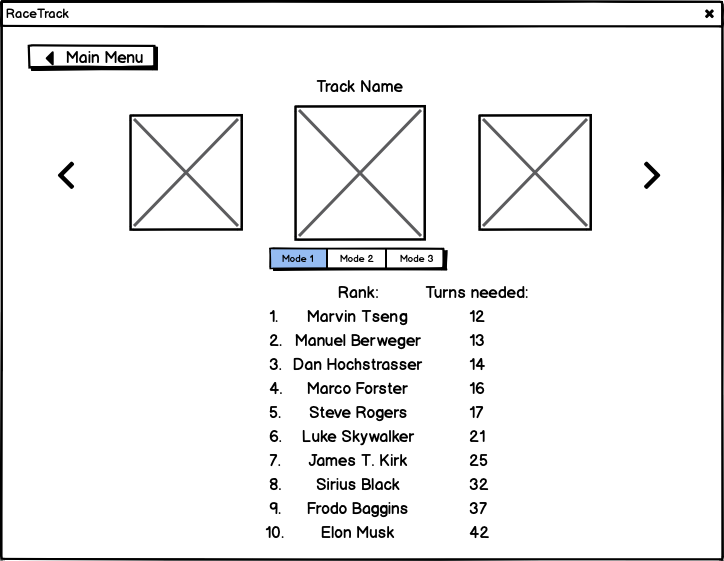
\includegraphics[width=8cm,keepaspectratio,center]{img/Use-Case-Model_UC1_UI-Sketch.png}
					\caption{UI Sketch of Use Case UC1}
				\end{figure}

		\subsubsection{Use Case UC4: Set Game Options}
			\textbf{Scope:} RaceTrack Game \\
			\textbf{Level:} User Goal \\
			\textbf{Primary Actor:} Player \\
			\textbf{Stakeholders and Interests:} \\
			Player: Wants to configure the options for the coming game session (UC7). \\
			\textbf{Preconditions:} No running game session at the moment. \\
			\textbf{Success Guarantee:} The preferences entered by the user are successfully applied to the created game session. \\
			\textbf{Frequency of Occurrence:} Once before each new game session.
			\newline
	
			\textbf{Main Success Scenario}
				\begin{enumerate}
					\item The player selects the \textit{New Game} entry in the menu.
					\item The player configures the settings for the new game session to his liking.
					\begin{enumerate}
						\item The player defines for each participating player the name and car color.
						\item The player defines how the game should handle crashes by selecting one out of three available game modes:
						\begin{enumerate}
							\item \textbf{Go Kart} : \textit{Continue with minimum velocity and no acceleration until the track is reached again}.
							\item \textbf{Formula One} : \textit{Retire from the race}.
							\item \textbf{Bobby Car} : \textit{Reset position to last valid point and reset velocity}.
						\end{enumerate}
						\item The player selects the track to be played on.
					\end{enumerate}
					\item The player finishes the setup for a new game session by clicking on the \textit{Start Game} button.
				\end{enumerate}
	
			\textbf{Alternative Flows}
				\begin{enumerate}
					\item When not all four player fields are filled out during game setup:
					\begin{enumerate}
						\item The game starts the session with only filled out players, players with no name are ignored.
					\end{enumerate}
				\end{enumerate}
	
			\textbf{Special Requirements}
				\begin{itemize}
					\item The settings must be easily understandable.
					\item Language internationalization on the text displayed.
					\item Only previously loaded tracks (UC13) can be chosen during the game setup.
				\end{itemize}
	
			\textbf{Technology and Data Variations List}
				\begin{itemize}
					\item The settings for the game session must be saved in a \textit{.rtsave} file.
					\item The \textit{.rtsave} file follows the JSON syntax.
				\end{itemize}

			\newpage
	
			\textbf{UI Sketch}
				\begin{figure}[H]
					\centering
					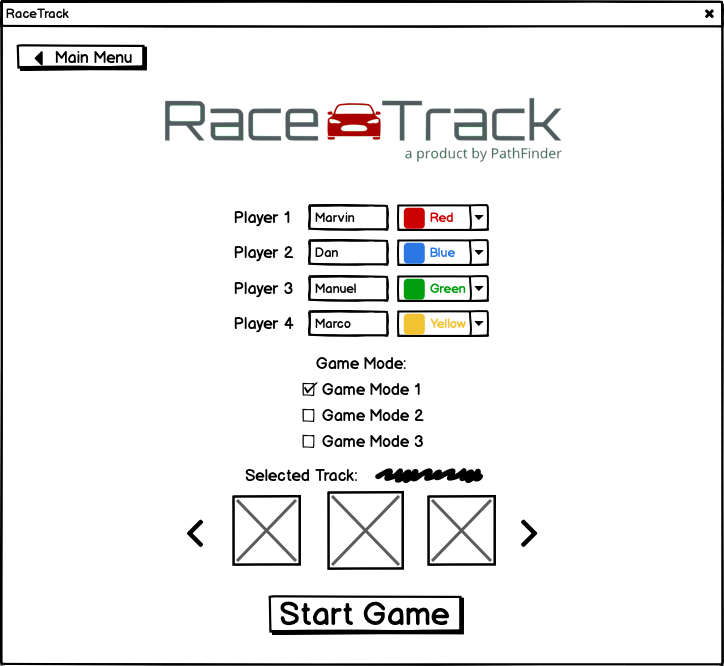
\includegraphics[width=9cm,keepaspectratio,center]{img/Use-Case-Model_UC4_UI-Sketch.png}
					\caption{UI Sketch for Use Case UC4}
				\end{figure}

		\subsubsection{Use Case UC10: Load Game Session}
			\textbf{Scope:} RaceTrack Game \\
			\textbf{Level:} User Goal \\
			\textbf{Primary Actor:} Player \\
			\textbf{Stakeholders and Interests:} \\
			Player: Wants to load a previously saved game session (UC11). \\
			\textbf{Preconditions:} A valid \textit{.rtsave} file containing all the necessary pieces of information to restore a past game session. \\
			\textbf{Success Guarantee:} A saved game session has been successfully loaded from a \textit{.rtsave} file. \\
			\textbf{Frequency of Occurrence:} Once per saved game session to load.
			\newline
		
			\textbf{Main Success Scenario}
				\begin{enumerate}
					\item The player is currently in the main menu of the game.
					\item The player selects \textit{Load Game} in the main menu.
					\item The player chooses one of the previously saved game sessions in the list to be loaded.
					\item The system loads the previously saved game session with the same state as saved.
				\end{enumerate}
		
			\textbf{Alternative Flows} \\
				\textit{No alternative flows present.} \\
		
			\textbf{Special Requirements}
				\begin{itemize}
					\item When the save file is loaded, the game state should be the same as before.
				\end{itemize}
		
			\textbf{Technology and Data Variations List}
				\begin{itemize}
					\item The resulting file that gets loaded must be a \textit{.rtsave} file.
					\item The \textit{.rtsave} file follows the JSON syntax.
				\end{itemize}
		
			\newpage

			\textbf{UI Sketch}
				\begin{figure}[H]
					\centering
					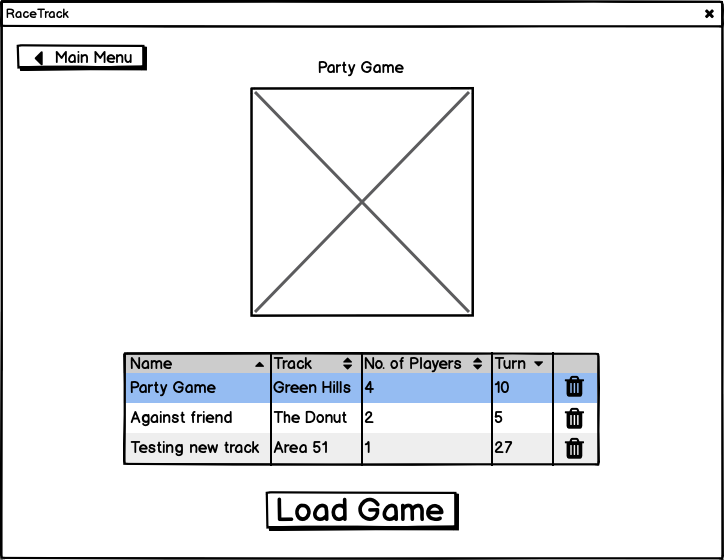
\includegraphics[width=9cm,keepaspectratio,center]{img/Use-Case-Model_UC15_UI-Sketch.png}
					\caption{UI Sketch for Use Case UC15}
				\end{figure}

		\subsubsection{Use Case UC11: Save Game Session}
			\textbf{Scope:} RaceTrack Game \\
			\textbf{Level:} User Goal \\
			\textbf{Primary Actor:} Player \\
			\textbf{Stakeholders and Interests:} \\
			Player: Wants to save a running game session (UC7) that hasn't been saved yet. \\
			\textbf{Preconditions:} A currently running game session (UC7). \\
			\textbf{Success Guarantee:} A running game session has been successfully saved in a \textit{.rtsave} file. \\
			\textbf{Frequency of Occurrence:} Usually once per game session.
			\newline
		
			\textbf{Main Success Scenario}
				\begin{enumerate}
					\item A game session is currently being played (UC7).
					\item The player selects the \textit{Save Game} entry in the menu of the game window.
					\item The game shows a success message to the player, that the session has been successfully saved.
				\end{enumerate}
		
			\textbf{Alternative Flows}
				\begin{enumerate}
					\item Any time the player wants to delete a previously saved game session:
					\begin{enumerate}
						\item The player is currently in the main menu of the game.
						\item The player selects \textit{Load Game} in the main menu.
						\item Instead, to \textit{load} the selected game session, the player chooses to \textit{delete} the saved game session.
					\end{enumerate}
				\end{enumerate}
		
			\textbf{Special Requirements}
				\begin{itemize}
					\item All information needed to save the current game state must be included in the save file.
				\end{itemize}
		
			\textbf{Technology and Data Variations List}
				\begin{itemize}
					\item The resulting file that gets created with a save must have the extension \textit{.rtsave}.
					\item The \textit{.rtsave} file follows the JSON syntax.
					\newpage
					\item Below is an example of such a \textit{.rtsave} file:
					\lstinputlisting[style=java,caption={Example of a Save File}]{img/Use-Case-Model_UC14_SaveFile-Example.rtsave}
				\end{itemize}
		
			\textbf{UI Sketch} \\~\\
				\textit{Already visible on the UI-Sketch for Use Case UC1: Play one Game Session.}

	\subsection{Minor Use Cases}

		\subsubsection{Use Case UC2: View Rules}
			Before the player starts playing the game, he wants to look at the rules of the game, so he knows how to play. The player opens the rule set in the main menu by clicking on the corresponding entry. The player should be able to easily understand the aim of the game by reading through the rules.

		\subsubsection{Use Case UC3: View Credits}
			The player is interested in the current game version and/or the developers of the game. In the main menu, he opens the credits dialog by clicking on the \textit{View Credits} button. In the credits dialog, he can easily determine the current game build and/or the names and contact information of the developers.

		\subsubsection{Use Case UC6: Reset Game Session}
			The player is not satisfied with the current state of the game, based on the moves the player has previously made. To reset his moves and start the game from the beginning, the player clicks on the \textit{Reset} button in the game window. Then the game will ask the player, if he is sure about the action. If he says yes, all elements in the game will be set to the initial state, otherwise, no changes will be made.

		